\newif\ifshowsolutions
\showsolutionstrue

\input{../preamble}

\chead{
  {\vbox{
      \vspace{2mm}
      \large
      Machine Learning \& Data Mining \hfill
      Caltech CS/CNS/EE 155 \hfill \\[1pt]
      Set 1\hfill
      January $6^{th}$, 2023 \\
    }
  }
}

\begin{document}
\pagestyle{fancy}



%%%%%%%%%%%%%%%%%%%%%%%%%%%%%%
% POLICIES
%%%%%%%%%%%%%%%%%%%%%%%%%%%%%%

\section*{Policies}
\begin{itemize}
	\item Due 9 PM PST, January $13^\text{th}$ on Gradescope. 
	\item You are free to collaborate on all of the problems, subject to the collaboration policy stated in the syllabus.
	\item If you have trouble with this homework, it may be an indication that you should drop the class.
	\item In this course, we will be using Google Colab for code submissions. You will need a Google account.
\end{itemize}

\section*{Submission Instructions}

\begin{itemize}
	\item Submit your report as a single .pdf file to Gradescope (entry code K3RPGE), under "Set 1 Report". 
	\item In the report, \textbf{include any images generated by your code} along with your answers to the questions.
	\item Submit your code by \textbf{sharing a link in your report} to your Google Colab notebook for each problem (see naming instructions below). Make sure to set sharing permissions to at least "Anyone with the link can view". \textbf{Links that can not be run by TAs will not be counted as turned in.} Check your links in an incognito window before submitting to be sure. 
	\item For instructions specifically pertaining to the Gradescope submission process, see \url{https://www.gradescope.com/get_started#student-submission}.
\end{itemize}


\section*{Google Colab Instructions}

For each notebook, you need to save a copy to your drive.

\begin{enumerate}
	\item Open the github preview of the notebook, and click the icon to open the colab preview.
	\item On the colab preview, go to File $\rightarrow$ Save a copy in Drive.
	\item Edit your file name to “lastname_firstname_originaltitle”, e.g.”yue_yisong_3_notebook_part1.ipynb”
\end{enumerate}

%%%%%%%%%%%%%%%%%%%%%%%%%%%%%%
% PROBLEM 1
%%%%%%%%%%%%%%%%%%%%%%%%%%%%%%

\newpage
\section{Basics [16 Points]}
\materials{lecture 1}

Answer each of the following problems with 1-2 short sentences.

\begin{problem}[2]
  What is a hypothesis set?
\end{problem}
\begin{solution}
  The hypothesis set is the space of all possible options for which a set of inputs can be mapped to a set of outputs. In other words it describes the space of both all the possible input options and output options together.
\end{solution}

\begin{problem}[2]
  What is the hypothesis set of a linear model?
\end{problem}
\begin{solution}
  For a linear model, the hypothesis set would be all inputs that can be described by vectors $x$, $w$, and $b$ in this formula:
  
  $$f(x|w,b) = w^Tx-b$$
\end{solution}

\begin{problem}[2]
  What is overfitting?
\end{problem}
\begin{solution}
  Overfitting is an issue of deep learning models in which the model, usually due to high variation in the training set or if the training set is too sparse, is heavily influenced by the noise within that set. It becomes highly specific to the training set and is not generalizable to other test data.
\end{solution}

\begin{problem}[2]
  What are two ways to prevent overfitting?
\end{problem}
\begin{solution}
  1. You can always validate that the model is working by running it with test data and getting an error estimate. If theres an inappropriate amount of error(high variance) the model is flawed.//
  2. If you don't have a test set, you can always split the training set and holdout a subset for testing and error estimation.
\end{solution}

\begin{problem}[2]
  What are training data and test data, and how are they used differently? Why should you never change your model based on information from test data?
\end{problem}
\begin{solution}
  Modifying your model based on test data effectively redefines (in philosophy) that test data as training data. Were you to re-run your model with that new incorporated training(previously test) data would cause the model to suffer from confirmation bias and inappropriately skew it.
\end{solution}

\begin{problem}[2]
  What are the two assumptions we make about how our dataset is sampled?
\end{problem}
\begin{solution}
  1. That the data is sampled independently from the same distribution and is thus, representative.\\
  2. The training set is large enough to accurately describe the ground truth distribution.
\end{solution}

\begin{problem}[2]
  Consider the machine learning problem of deciding whether or not an email is spam. What could $X$, the input space, be? What could $Y$, the output space, be?
\end{problem}
\begin{solution}
  The input space could be a vector with binary (0 or 1) elements with each element corresponding to the presence or absence of a word. The output space can also be binary(in this case we use +1 or -1 though this can just be convention) to indicate whether the whole email is spam or not spam.
\end{solution}

\begin{problem}[2]
  What is the $k$-fold cross-validation procedure?
\end{problem}
\begin{solution}
    With limited data, it helps to separate the training set into k parts. k-1 will be used for training and that last subset will be used for testing. This can be done iteratively, holding out each subset in k and training with the rest. In this way you can get a sense of the error associated with all parts of the training data without need for separate test data.
\end{solution}



%%%%%%%%%%%%%%%%%%%%%%%%%%%%%%
% PROBLEM 2
%%%%%%%%%%%%%%%%%%%%%%%%%%%%%%

\newpage
\section{Bias-Variance Tradeoff [34 Points]}
\materials{lecture 1}

\begin{problem}[5]
  Derive the bias-variance decomposition for the squared error loss function. That is, show that for a model $f_S$ trained on a dataset $S$ to predict a target $y(x)$ for each $x$,
  \begin{align*}
    \E_S \left[E_\text{out}\left(f_S\right)\right] = \E_x[\Bias(x) + \Var(x)]
  \end{align*}
  given the following definitions:
  \begin{align*}
    F(x) &= \E_S\left[f_S(x) \right] \\
    E_\text{out}(f_S) &= \E_x\left[\left(f_S(x) - y(x)\right)^2\right] \\
    \Bias(x) &= (F(x) - y(x))^2 \\
    \Var(x) &= \E_S\left[(f_S(x)-F(x))^2\right]
  \end{align*}
\end{problem}

\begin{solution}
  Starting from:  
  $$E_{out}(fs) = E_x[(fs(x)-y(x))^2]$$
and 
  $$F_(x) = E_s[fs(x)]$$
We can get to 
  $$F(x) = E_s[E_x[(fs(x)-y(x))^2] = E_x[E_s[(fs(x)-y(x))^2]]$$
So let's isolate the $E_s$ part:
  $$E_s[(fs(x)-y(x))^2] = E_s[(fs(x)-F(x) + F(x) - y(x))^2]$$
  
  $$= E_s[(fs(x)-F(x))^2 + (F(x) - y(x))^2 + 2(fs(x)-F(x)(F(x) - y(x))]$$

  $$= E_s[(fs(x)-F(x))^2] + (F(x) - y(x))^2$$

  The first portion, 
  
  $$E_s[(fs(x)-F(x))^2]$$

  we define as Var(x), and the second

  $$(F(x) - y(x))^2$$

  we define as Bias(x), thus we have that:

  $$E_s[E_{out}(fs(x)] = E_x[Var(x) + Bias(x)]$$
\end{solution}

In the following problems you will explore the bias-variance tradeoff by producing learning curves for polynomial regression models.

A \emph{learning curve} for a model is a plot showing both the training error and the cross-validation error as a function of the number of points in the training set. These plots provide valuable information regarding the bias and variance of a model and can help determine whether a model is over-- or under--fitting.

\emph{Polynomial regression} is a type of regression that models the target $y$ as a degree--$d$ polynomial function of the input $x$. (The modeler chooses $d$.)  You don't need to know how it works for this problem, just know that it produces a polynomial that attempts to fit the data.

\begin{problem}[14]
    Use the provided \texttt{2_notebook.ipynb} Jupyter notebook to enter your code for this question. This notebook contains examples of using NumPy's polyfit and polyval methods, and scikit-learn's KFold method; you may find it helpful to read through and run this example code prior to continuing with this problem. Additionally, you may find it helpful to look at the documentation for scikit-learn's learning_curve method for some guidance.

The dataset \texttt{bv_data.csv} is provided and has a header denoting which columns correspond to which values. Using this dataset, plot learning curves for 1st--, 2nd--, 6th--, and 12th--degree polynomial regression (4 separate plots) by following these steps for each degree $d \in \{1, 2, 6, 12\}$:

  \begin{enumerate}
    \item For each $N \in \{20, 25, 30, 35, \cdots, 100\}$:
    \begin{enumerate}[i.]
      \item Perform 5-fold cross-validation on the first $N$ points in the dataset (setting aside the other points), computing the both the training and validation error for each fold. 
      \begin{itemize}
        \item Use the mean squared error loss as the error function.
        \item Use NumPy's polyfit method to perform the degree--$d$ polynomial regression and NumPy's polyval method to help compute the errors.  (See the example code and \href{https://docs.scipy.org/doc/NumPy/reference/routines.polynomials.poly1d.html}{NumPy documentation} for details.)
        \item When partitioning your data into folds, although in practice you should randomize your partitions, for the purposes of this set, simply divide the data into $K$ contiguous blocks.
      \end{itemize}
      \item Compute the average of the training and validation errors from the 5 folds.
    \end{enumerate}
    \item Create a learning curve by plotting both the average training and validation error as functions of $N$. \textit{Hint: Have same y-axis scale for all degrees $d$.}
  \end{enumerate}

\end{problem}
\begin{solution}
https://colab.research.google.com/drive/1Ruu4LfY8ZMlcTOPT_B0JJLydgZd14gW4?usp=sharing

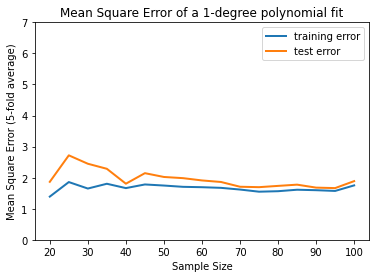
\includegraphics{set1/images/Unknown-6.png}\\
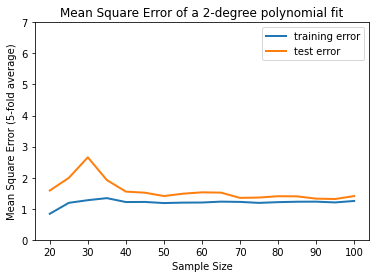
\includegraphics{set1/images/Unknown-7.png}\\
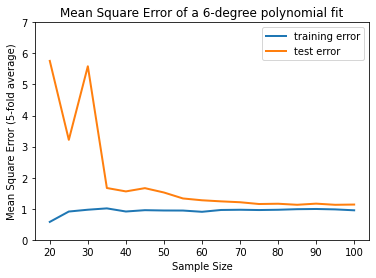
\includegraphics{set1/images/Unknown-8.png}\\
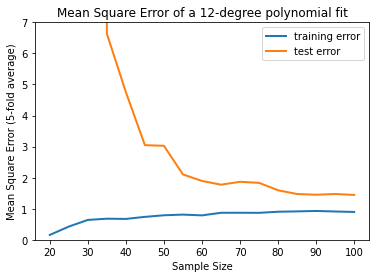
\includegraphics{set1/images/Unknown-9.png}


  \end{solution}

\begin{problem}[3]
  Based on the learning curves, which polynomial regression model (i.e. which degree polynomial) has the highest bias? How can you tell?
\end{problem}
\begin{solution}
The bias is highest in the 1st degree polynomial fit since the overall training error has a higher baseline than the rest
\end{solution}

\begin{problem}[3]
  Which model has the highest variance? How can you tell?
\end{problem}
\begin{solution}
  The 12th degree polynomial fit has the highest variance since the test error is much higher than the rest and relative to the training set
\end{solution}

\begin{problem}[3]
  What does the learning curve of the quadratic model tell you about how much the model will improve if we had additional training points?
\end{problem}
\begin{solution}
The learning curve error becomes inconsequential after a certain number of data points. Thus, incorporating more data into the training model doesn't necessarily increase its accuracy and may be an inefficient use of resources.
\end{solution}

\begin{problem}[3]
  Why is training error generally lower than validation error?
\end{problem}
\begin{solution}
  Because the model is literally trained on the training set. Therefore, the model will always recapitulate the training data more robustly. It's like asking "Why does a baby like their Mom better than a stranger?". 
\end{solution}

\begin{problem}[3]
  Based on the learning curves, which model would you expect to perform best on some unseen data drawn from the same distribution as the training data, and why?
\end{problem}
\begin{solution}
  The 6th degree polynomial fit has the lowest overall error and the validation error closely approximates the training error after maybe 70 data points, therefore would perform the best.
\end{solution}




%%%%%%%%%%%%%%%%%%%%%%%%%%%%%%
% PROBLEM 3
%%%%%%%%%%%%%%%%%%%%%%%%%%%%%%

\newpage
\section{Stochastic Gradient Descent [34 Points]}
\materials{lecture 2}

Stochastic gradient descent (SGD) is an important optimization method in machine learning, used everywhere from logistic regression to training neural networks. In this problem, you will be asked to analyze gradient descent and implement SGD for linear regression using the squared loss function. Then, you will analyze how several parameters affect the learning process.

\begin{problem}[3]
    To verify the convergence of our gradient descent algorithm, consider the task of minimizing a function $f$ (assume that $f$ is continuously differentiable). Using Taylor's theorem, show that if $x'$ is a local minimum of $f$, then $\nabla f(x') = 0$. 
\end{problem}
\begin{hint}
  First-order Taylor expansion gives that for any $x, h \in \mathbb{R}^n$, there exists $c \in (0, 1)$ such that $f(x + h) = f(x) + \nabla f(x + c\cdot h)^T h$.
  
\end{hint}
\begin{solution}
Starting from above and let's imagine we're on some kind of convex curve. Now let's put our pies in the sky(that's where I like 'em) and assume that $\nabla f(x') \not= 0$ shocking right? \\

We can define a vector $p=-\nabla f(x')$ and say this:

$$p^T \nabla f(x') = -|\nabla f(x')|^2 < 0$$\\

we can then walk along our curve some $t \in [0,T]$ (we know we can do this because its continuous differentiable near x' so ha).
\\
then we have:
$$p^T \nabla f(x'+tp) < 0$$

and by using the theorem (Taylor's Version) we can rewrite this as

$$p^T \nabla f(x'+tp) = f(x') + t p^T \nabla f(x'+tp)$$

this lends itself to saying that:
$$f(x'+tp) < f(x')$$ for ALL $t \in (0,t)$

So we've found that at an x' and moving some distance away from this x' in a specific direction will lead to a decrease in f, suggesting that this is NOT a local minimum at x'. This is called a contradiction, the presence of a contradiction proves the rule.

\end{solution}

Linear regression learns a model of the form:
\begin{align*}
  f(x_1, x_2, \cdots, x_d) = \left(\sum_{i=1}^d w_i x_i\right) + b
\end{align*}

\begin{problem}[1]
  We can make our algebra and coding simpler by writing $f(x_1, x_2, \cdots, x_d) = \mathbf{w}^T\mathbf{x}$ for vectors $\mathbf{w}$ and $\mathbf{x}$.  But at first glance, this formulation seems to be missing the bias term $b$ from the equation above.  How should we define $\mathbf{x}$ and $\mathbf{w}$ such that the model includes the bias term?
\end{problem}
\begin{hint}
  Include an additional element in $\mathbf{w}$ and $\mathbf{x}$.
\end{hint}
\begin{solution}
  We can add some term $w_b$ and $x_b$ which can be found in the vectors $w$ and $x$ such that some part of the operation for $w^Tx$ is:
  $$w_b x_b + w_1 x_1 + ... + w_d x_d$$

  If we set $x_b = 1$ then we can generate a bias term specified purely by the weight vector.
\end{solution}

Linear regression learns a model by minimizing the squared loss function $L$, which is the sum across all training data $\{(\mathbf{x}_1, y_1),\cdots,(\mathbf{x}_N, y_N)\}$ of the squared difference between actual and predicted output values:
\[L(f) = \sum_{i=1}^N (y_i - \mathbf{w}^T\mathbf{x}_i)^2\]

\begin{problem}[2]
  Both GD and SGD uses the gradient of the loss function to make incremental adjustments to the weight vector $\mathbf{w}$. Derive the gradient of the squared loss function with respect to $\mathbf{w}$ for linear regression. Explain the difference in computational complexity in 1 update of the weight vector between GD and SGD. 
\end{problem}
\begin{solution}
  We can take the derivative of L(f):
    $$L(f) = \sum_{i=1}^N (y_i - \mathbf{w}^T\mathbf{x}_i)^2$$

    Lets say 
    $$h = y_i - \mathbf{w}^T\mathbf{x}_i$$
    and
    $$h' = -x_i$$

    $$L(f) = \sum_{i=1}^N (h)^2$$

    via chain rule
    $$L' (f) = 2(h) h'$$
    
    $$L' (f)=\sum^{N}_{i=1} 2(y_i-w^Tx_i)(- x_i) $$
    $$L' (f)=\sum^{N}_{i=1} 2x_i(w^Tx_i-y_i)$$

    \\

    The difference in complexity is simply iterative. For N data points, GD requires N calculations of L'(f) whereas with SGD, we need some random subset of N in order to compute a similar update.
\end{solution}

The following few problems ask you to work with the first of two provided Jupyter notebooks for this problem, \texttt{3_notebook_part1.ipynb}, which includes tools for gradient descent visualization. This notebook utilizes the files \texttt{sgd_helper.py} and \texttt{multiopt.mp4}, but you should not need to modify either of these files. 

For your implementation of problems D-F, \textbf{do not} consider the bias term.

\begin{problem}[6]
  Implement the \texttt{loss}, \texttt{gradient}, and \texttt{SGD} functions, defined in the notebook, to perform SGD, using the guidelines below:

  \begin{itemize}
    \item Use a squared loss function.
    \item Terminate the SGD process after a specified number of epochs, where each epoch performs one SGD iteration for each point in the dataset.
    \item It is recommended, but not required, that you shuffle the order of the points before each epoch such that you go through the points in a random order. You can use \texttt{numpy.random.permutation}.
    \item Measure the loss after each epoch. Your \texttt{SGD} function should output a vector with the loss after each epoch, and a matrix of the weights after each epoch (one row per epoch). Note that the weights from all epochs are stored in order to run subsequent visualization code to illustrate SGD.
  \end{itemize}
\end{problem}
\begin{solution}
See code.\\ %This does not need to be changed.
https://drive.google.com/file/d/1HkxEZQL79CDc4ehbmczhO_YaVt3U6LXA/view?usp=sharing
\end{solution}

\begin{problem}[2]
  Run the visualization code in the notebook corresponding to problem D. How does the convergence behavior of SGD change as the starting point varies? How does this differ between datasets 1 and 2? Please answer in 2-3 sentences.
\end{problem}
\begin{solution}
Both datasets feature SGD convergence towards the global minimum of the system regardless of the starting point. It's important to note that the system is a simple convex plane in both cases and therefore has only one minimum, respectively.
\end{solution}

\begin{problem}[6]
  Run the visualization code in the notebook corresponding to problem E. One of the cells---titled "Plotting SGD Convergence"---must be filled in as follows. Perform SGD on dataset 1 for each of the learning rates $\eta \in \{10^{-6}, 5 \cdot 10^{-6}, 10^{-5}, 3 \cdot 10^{-5}, 10^{-4}\}$. On a single plot, show the training error vs. number of epochs trained for each of these values of $\eta$. What happens as $\eta$ changes?
\end{problem}

\begin{solution}
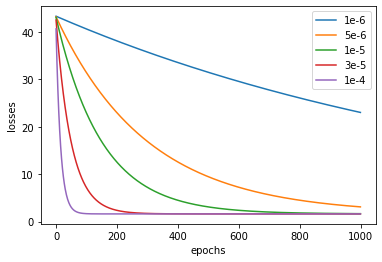
\includegraphics{set1/images/Unknown-10.png}\\ 
\\
As $\eta$ changes we see that the time it takes for full convergence takes much longer, therefore may not be reasonable in the time frame of our model.
\end{solution}


The following problems consider SGD with the larger, higher-dimensional dataset, \texttt{sgd_data.csv}. The file has a header denoting which columns correspond to which values. For these problems, use the Jupyter notebook \texttt{3_notebook_part2.ipynb}.

For your implementation of problems G-I, \textbf{do} consider the bias term using your answer to problem A.

\begin{problem}[6]
  Use your SGD code with the given dataset, and report your final weights. Follow the guidelines below for your implementation:

  \begin{itemize}
    \item Use $\eta = e^{-15}$ as the step size.  
    \item Use $\mathbf{w} = [0.001, 0.001, 0.001, 0.001]$ as the initial weight vector and $b = 0.001$ as the initial bias.
    \item Use at least 800 epochs.
    \item You should incorporate the bias term in your implementation of SGD and do so in the vector style of problem A.
    \item Note that for these problems, it is no longer necessary for the \texttt{SGD} function to store the weights after all epochs; you may change your code to only return the final weights.
  \end{itemize}
  %$\epsilon$ here is a measure of how much change in error there is compared to the initial error in the epoch. Calculate the change in error every epoch and compare it to the change in error from the first epoch. If new change/initial change is less than $\epsilon$, stop the training. $\eta$ is the factor by which you multiply the gradient in each step of the descent, and $\mathbf{w}$ is the initial weight vector.
\end{problem}
\begin{solution}
https://drive.google.com/file/d/1K_gI8mB9AxjRMh4mdWWp5sLbuzAaGdMm/view?usp=sharing
\\
\\
The final weights are:
[ -5.97853793   3.988393   -11.85700887   8.91129577  -0.22789823]
\end{solution}

\begin{problem}[2]
  Perform SGD as in the previous problem for each learning rate $\eta$ in \[\{e^{-10}, e^{-11}, e^{-12}, e^{-13}, e^{-14}, e^{-15}\},\] and calculate the training error at the beginning of each epoch during training.  On a single plot, show training error vs. number of epochs trained for each of these values of $\eta$. Explain what is happening.
\end{problem}
\begin{solution}
  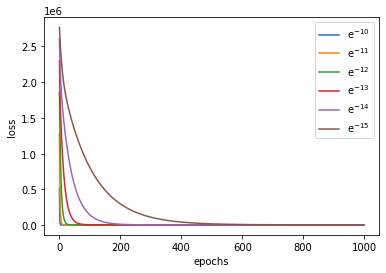
\includegraphics{set1/images/Unknown-11.png}\\
  \\
  We can see that the model converges fastest with the highest learning rate and that all must reach convergence within 1000 epochs
\end{solution}


\begin{problem}[2]
  The closed form solution for linear regression with least squares is \[\mathbf{w} = \left(\sum_{i=1}^N \mathbf{x_i}\mathbf{x_i}^T\right)^{-1}\left(\sum_{i=1}^N \mathbf{x_i}y_i\right).\]  Compute this analytical solution.  Does the result match up with what you got from SGD?
\end{problem}
\begin{solution}
   The analytically computed weights are:
  
  [ -5.99157048   4.01509955 -11.93325972   8.99061096  -0.31644251]
  \\
  This is quite close to the approximation via SGD however there is small variation in the output.
\end{solution}

Answer the remaining questions in 1-2 short sentences.

\begin{problem}[2]
  Is there any reason to use SGD when a closed form solution exists?
\end{problem}
\begin{solution}
In this case there is no need to compute the SGD since it is computationall expensive. A closed form would always preclude the need for optimization.
\end{solution}

\begin{problem}[2]
  Based on the SGD convergence plots that you generated earlier, describe a stopping condition that is more sophisticated than a pre-defined number of epochs.
\end{problem}
\begin{solution}
  A more appropriate approach, depending on how computationally heavy the optimization is, is to define a maximum training error. As long as the error is less than that maximum threshold that you deem acceptable, that would be more appropriate as the end goal of this approach is to get a working model.
\end{solution}


%%%%%%%%%%%%%%%%%%%%%%%%%%%%%%
% PROBLEM 4
%%%%%%%%%%%%%%%%%%%%%%%%%%%%%%

\newpage
\section{The Perceptron [16 Points]}
\materials{lecture 2}

The perceptron is a simple linear model used for binary classification. For an input vector $\mathbf{x} \in \mathbb{R}^d$, weights $\mathbf{w} \in \mathbb{R}^d$, and bias $b \in \mathbb{R}$, a perceptron $f: \mathbb{R}^d \rightarrow \{-1,1\}$ takes the form
\begin{align*}
  f(\mathbf{x}) = \operatorname{sign}\left(\left(\sum_{i=1}^d w_i x_i\right) + b \right)
\end{align*}

The weights and bias of a perceptron can be thought of as defining a hyperplane that divides $\mathbb{R}^d$ such that each side represents an output class. For example, for a two-dimensional dataset, a perceptron could be drawn as a line that separates all points of class $+1$ from all points of class $-1$.

The PLA (or the Perceptron Learning Algorithm) is a simple method of training a perceptron. First, an initial guess is made for the weight vector $\mathbf{w}$. Then, one misclassified point is chosen arbitrarily and the $\mathbf{w}$ vector is updated by
\begin{align*}
  \mathbf{w}_{t+1} &= \mathbf{w}_t + y(t)\mathbf{x}(t) \\
  b_{t + 1} &= b_t + y(t),
\end{align*}

where $\mathbf{x}(t)$ and $y(t)$ correspond to the misclassified point selected at the $t^\text{th}$ iteration.
This process continues until all points are classified correctly.

The following few problems ask you to work with the provided Jupyter notebook for this problem, titled \texttt{4_notebook.ipynb}. This notebook utilizes the file \texttt{perceptron_helper.py}, but you should not need to modify this file.

\begin{problem}[8]
  The graph below shows an example 2D dataset. The $+$ points are in the $+1$ class and the $\circ$ point is in the $-1$ class. 

  \begin{figure}[H]
    \centering
    \includegraphics[width=0.4\textwidth]{images/perceptron.png}
    \caption{The green $+$ are positive and the red $\circ$ is negative}
    \label{fig:figure1}
  \end{figure}
  
 Implement the \texttt{update_perceptron} and \texttt{run_perceptron} methods in the notebook, and perform the perceptron algorithm with initial weights $w_1 = 0, w_2 = 1, b = 0$.

  Give your solution in the form a table showing the weights and bias at each timestep and the misclassified point $([x_1,x_2],y)$ that is chosen for the next iteration's update. You can iterate through the three points in any order. Your code should output the values in the table below; cross-check your answer with the table to confirm that your perceptron code is operating correctly.

  \begin{table}[H]
    \centering

    \begin{tabular}{l|lll|ll|l}
    \hline

    \hline
    $t$ & $b$ & $w_1$ & $w_2$ & $x_1$ & $x_2$ & $y$ \\
    \hline
      0  &  0 & 0 & 1  & 1 & -2 & +1\\
      1  &  1 & 1 & -1 & 0 & 3 & +1\\
      2  &  2 & 1 & 2 & 1 & -2 & +1\\
      3  &  3 & 2 & 0 \\
    \hline
    \end{tabular}
  \end{table}
  
  Include in your report both: the table that your code outputs, as well as the plots showing the perceptron's classifier at each step (see notebook for more detail).
  
  
\end{problem}
\begin{solution}
https://drive.google.com/file/d/1xQSa-HrBEE2z4ReVrmHtzkc1LTP05rCs/view?usp=sharing\\
\\
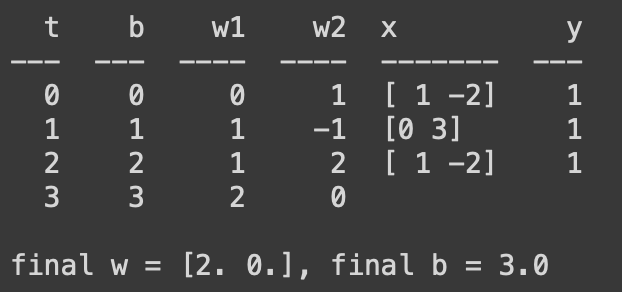
\includegraphics{set1/images/Unknown-14.png}
\\
\\
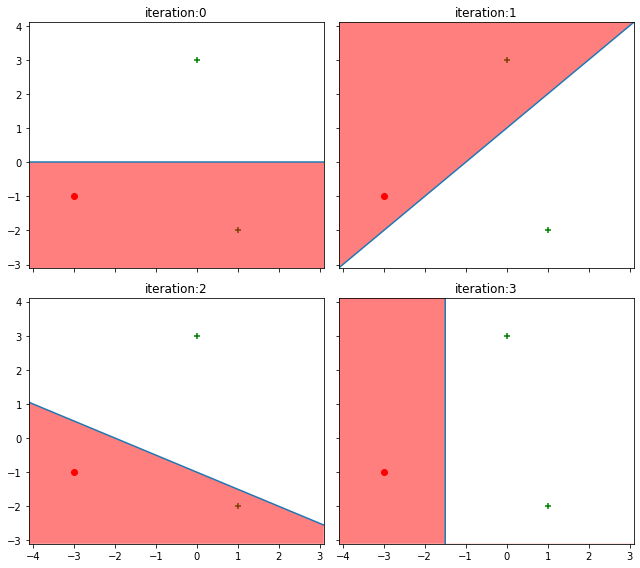
\includegraphics[width=10cm, height=10cm]{set1/images/Unknown-13.png}

\end{solution}

\begin{problem}[4]
  A dataset $S = \{(\mathbf{x}_1, y_1),\cdots,(\mathbf{x}_N, y_N)\} \subset \mathbb{R}^d \times \mathbb{R}$ is \emph{linearly separable} if there exists a perceptron that correctly classifies all data points in the set. In other words, there exists a hyperplane that separates positive data points and negative data points.

  In 2D space, what is the minimum size of a dataset that is not linearly separable, such that no three points are collinear? How about the minimum size of a dataset in 3D that is not linearly separable, such that no four points are coplanar, and given no 2D subspace contains a non-linearly-separable subset? Please limit your explanation to a few lines - you should justify but not prove your answer.

  Finally, how does this generalize to N-dimension, in which no $<N$-dimensional subspace contains a non-linearly-separable subset? More precisely, in N-dimensional space, what is the minimum size of a dataset that is not linearly separable, such that no $N+1$ points are on the same hyperplane? For the $N$-dimensional case, you may state your answer without proof or justification.

\end{problem}
\begin{solution}
For a 2D space, the minimum is 4 points assuming non-colinearity in 3. Imagine a 2 points in a 2D space and let's assume they belong to the positive group. Now let's draw a line connecting these two points. Add another two points on *either side* of this line and make these the negative group. You've now created a 2D space where the two groups are not linearly separable no matter what line you draw.\\
\\
Same rules as above, the minimum would be 5. Let's draw 3 points in space corresponding to the positive group. Now draw a plane connecting these 3 points. Once again, draw 2 points, each normal to one face of the plane (i.e. one up, one down). We can see another set of nonlinearly separable points.
\\
We can generalize this to say that $N+2$ is the minimum number of points where $N$ is the dimension of the space. I can't and won't provide proof. :)
\end{solution}

\begin{problem}[2]
  Run the visualization code in the Jupyter notebook section corresponding to question C (report your plots). Assume a dataset is \emph{not} linearly separable. Will the Perceptron Learning Algorithm ever converge? Why or why not?
\end{problem}
\begin{solution}
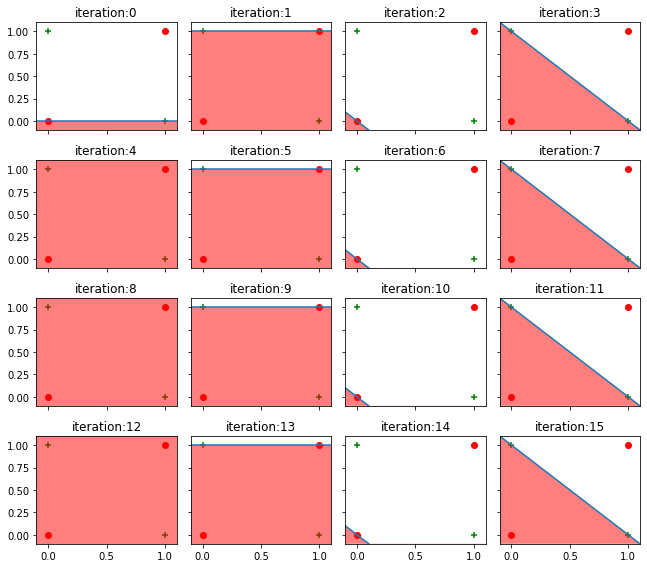
\includegraphics[width=10cm, height=10cm]{set1/images/Unknown-15.png}\\
\\
We can see that this non linearly separable group will not converge. There will always be some number of points that are misclassified leading to error in our algorithm and thus, iterative updates.
\end{solution}

\begin{problem}[2]
How does the convergence behavior of the weight vector differ between the perceptron and SGD algorithms? Think of comparing, at a high level, their smoothness and whether they always converge (You don't need to implement any code for this problem.)
\end{problem}
\begin{solution}
The perceptron works on non-continuous functions due to the nature of using a subgradient, thus not requiring linear separability to run and optimize. Conversely, the SGD algorithm relies on a continuously differentiable function(smooth) in order to solve and optimize. In this case the smoother the better.
\end{solution}
\end{document}
